\documentclass[]{article}
\usepackage{amsmath}
\usepackage{graphicx}
\usepackage{float}
\usepackage{mwe}    % loads »blindtext« and »graphicx«
\usepackage{subfig}
\usepackage{url}
%opening
\title{Assignment - Constrained optimization\\Interior Point Method applied to linear programming
	problems}
\author{Matteo Bunino}

\begin{document}

\maketitle

\section{Problem definition}
The Predictor-Corrector is an Interior Point Method built to iteratively solve a nonlinear system of equations, obtained by defining the KKT condition for the pair primal-dual problem.\\
The linear system to solve is:
\begin{equation*}
	F(x,\lambda, s) = 
	\begin{bmatrix}
	Ax-b \\[0.3em]
	s+A^T\lambda-c \\[0.3em]
	XSe          
	\end{bmatrix}
	=0
\end{equation*}

According to Newton method for nonlinear system of equation, the system can be locally linearized and solved. To linearize this system is necessary to compute the Jacobian of $F$ at each iteration and solve the linear system:
\begin{equation*}
	F'(x_k,\lambda_k, s_k) \cdot 
	\begin{pmatrix}
	\Delta x_k \\[0.3em]
	\Delta \lambda_k \\[0.3em]
	\Delta s_k           
	\end{pmatrix}
	+ F(x_k,\lambda_k, s_k)=0\\
\end{equation*}
\begin{equation*}
\begin{pmatrix}
A & 0 & 0 \\[0.3em]
0 & A^T & I \\[0.3em]
S_k & 0 & X_k           
\end{pmatrix}
\cdot 
\begin{pmatrix}
\Delta x_k \\[0.3em]
\Delta \lambda_k \\[0.3em]
\Delta s_k           
\end{pmatrix}
+ F(x_k,\lambda_k, s_k)=0\\
\end{equation*}
\\
Where $X_k=diag(x_k)$ and $S_k=diag(s_k)$.\\
Interior point methods are variants of Newton method that guarantee that each iterate $(x_k, \lambda_k, s_k)$ satisfy the constraint $x_k, s_k\geq0$.
\pagebreak
\section{Problem data}
$A=(1, \dots 1)\in \Re^{1*n}$, \\
$b = 1$,\\
$c \in \Re^n:c_i=a$ if $i$ is odd, otherwise 1.\\
$x \in \Re^n$.\\\\
After having built the sparse jacobian of F, using the command spy() it's possible to inspect its structure:

\begin{figure}[h]
	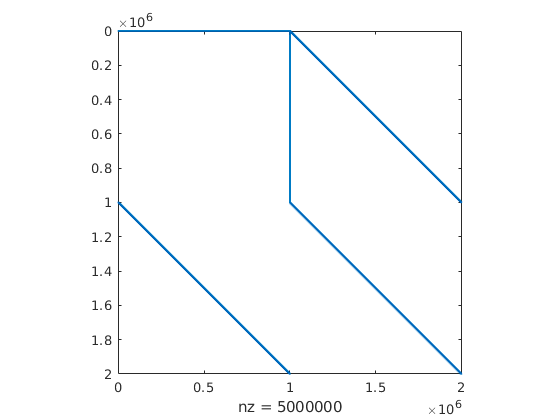
\includegraphics[width=12cm]{code/AA.png}
\end{figure}

Using the command [R,p] = chol(J) it's possible to notice, thanks to the value of p, that the matrix isn't positive definite. Hence I could not use: gradient method, conjugate gradient or Cholesky decomposition.\\
Since this matrix isn't symmetric, I couldn't use the LDL decomposition neither.\\
Hence I used two different strategies: LU decomposition and system reduction.

\subsection{LU decomposition}
As suggested in its documentation, Matlab has a specific implementation of the command lu() which is efficient for sparse matrices: [L,U,P,Q] = lu(A).\\
This command makes the $PAQ = LU$ decomposition of a matrix, where $L,U$ are triangular matrices and $P,Q$ permutation matrices.\\
A linear system can be solved with this factorization the following way:
\begin{equation*}
\begin{split}
PA = LUQ^{-1}\\
Ax = b \implies PAx = Pb\\
LUQ^{-1}x = Pb
\end{split}
\end{equation*}
\begin{enumerate}
	\item $Lz = Pb \implies z$
	\item $Uy = z \implies y$
	\item $Q^{-1}x = y \implies x = Qy$
\end{enumerate}
The advantage of this method is that we have to factorize the jacobian of F only once per each iteration and we can use it to solve two linear systems where only the right hand vector has changed.\\\\
Matlab lu() result:
\begin{figure}[!ht]
	\subfloat[L matrix\label{subfig-1:dummy}]{%
		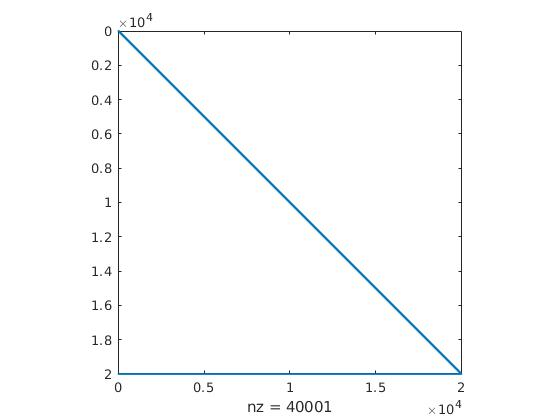
\includegraphics[width=0.5\textwidth]{code/L.jpg}
	}
	\hfill
	\subfloat[U matrix\label{subfig-2:dummy}]{%
		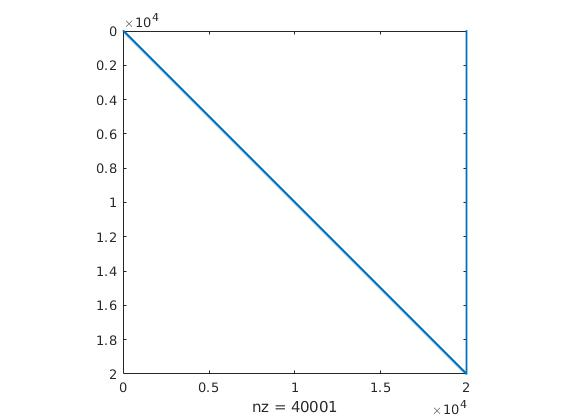
\includegraphics[width=0.5\textwidth]{code/U.jpg}
	}\\
	\subfloat[P matrix\label{subfig-3:dummy}]{%
		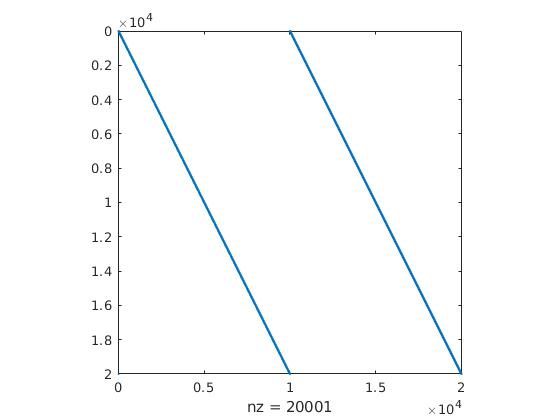
\includegraphics[width=0.5\textwidth]{code/P.jpg}
	}
	\hfill
	\subfloat[Q matrix\label{subfig-4:dummy}]{%
		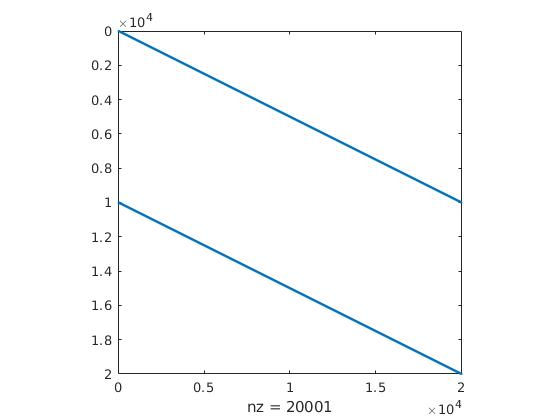
\includegraphics[width=0.5\textwidth]{code/Q.jpg}
	}
	\caption{As we can see, that matlab command is able to preserve (if possible) the sparse structure of the matrices.}
	\label{fig:dummy}
\end{figure}
\subsection{System reduction}
Analyzing the structure of the block matrix, we can notice that it's possible to make some reductions. Rewriting the left hand part in a more compact way:
\begin{equation*}
\begin{pmatrix}
A & 0 & 0 \\[0.3em]
0 & A^T & I \\[0.3em]
S_k & 0 & X_k           
\end{pmatrix}
\cdot 
\begin{pmatrix}
\Delta x_k \\[0.3em]
\Delta \lambda_k \\[0.3em]
\Delta s_k           
\end{pmatrix}
= 
\begin{pmatrix}
r_a \\[0.3em]
r_b \\[0.3em]
r_c         
\end{pmatrix}
\end{equation*}
From the second equation is possible to to write: $\Delta s = r_b - A^T\Delta\lambda$.\\
Since $X$ is invertible ($x > 0$ is guarateed by the IPM) it's possible to eliminate $I$ from the block matrix: $R_1 = R_1 -X^{-1}R_3$ ($R_i$ is the $i$-th row):
\begin{equation*}
\begin{pmatrix}
A & 0 & 0 \\[0.3em]
-X^{-1}S & A^T & 0 \\[0.3em]
S & 0 & X           
\end{pmatrix}
\cdot 
\begin{pmatrix}
\Delta x \\[0.3em]
\Delta \lambda \\[0.3em]
\Delta s           
\end{pmatrix}
= 
\begin{pmatrix}
r_a \\[0.3em]
r_b-X^{-1}r_c \\[0.3em]
r_c         
\end{pmatrix}
\end{equation*}
Now $\Delta s$ can be extracted from the system: $\Delta s = X^{-1}r_c-X^{-1}S\Delta x$, obtaining:
\begin{equation*}
	\begin{pmatrix}
	A & 0\\
	-X^{-1}S & A^T
	\end{pmatrix}
	\cdot
	\begin{pmatrix}
	\Delta x \\[0.3em]
	\Delta \lambda \\[0.3em]
	\end{pmatrix}
	=
	\begin{pmatrix}
	r_a\\
	r_b-X^{-1}r_c
	\end{pmatrix}
\end{equation*}
Since $S$ is invertible ($s > 0$ is guarateed by the IPM) it's possible to eliminate $A$ from the block matrix: $R_1 = R_1 +AS^{-1}XR_2$ ($R_i$ is the $i$-th row):
\begin{equation*}
\begin{pmatrix}
0 & AS^{-1}XA^T\\
-X^{-1}S & A^T
\end{pmatrix}
\cdot
\begin{pmatrix}
\Delta x \\[0.3em]
\Delta \lambda \\[0.3em]
\end{pmatrix}
=
\begin{pmatrix}
r_a + AS^{-1}X(r_b-X^{-1}r_c)\\
r_b-X^{-1}r_c
\end{pmatrix}
\end{equation*}
From which we can obtain:
\begin{equation*}
	\begin{split}
	AS^{-1}XA^T\Delta\lambda&=r_a+AS^{-1}Xr_b-AS^{-1}r_c\\
	\Delta s &= r_b-A^T\Delta \lambda\\
	\Delta x &=-S^{-1}X(r_b-A^T\Delta \lambda - X^{-1}r_c)\\
	&=-S^{-1}X(\Delta s - X^{-1}r_c)\\
	&= S^{-1}r_c-S^{-1}X\Delta s
	\end{split}
\end{equation*}
The matrix $AS^{-1}XA^T \in \Re^{mxm}$ is a real number, since in this case $m=1$. This makes the computation of the system trivial.
\pagebreak
\section{Results}
The reduction of the Jacobian was motivate by the unfeasibility of the problem when n gets very large (1M in this case), leading to a memory error.\\
To solve the problem with a direct method suited for an indefinite non symmetric matrix I used the LU decomposition, which is slightly less time consuming than the Gaussian elimination and it doesn't need to be computed twice for each iteration (we have to solve two linear systems with the same coefficient matrix).\\\\
What improved the performances, indeed, was the chosen starting point. We know that it's not necessary for the starting point to exactly fulfill all the first order optimality conditions, but just $x, s > 0$.\\
I tried 3 starting configurations:
\begin{enumerate}
	\item [a.]$x=ones(n,1)$, $s=ones(n,1)$, $\lambda = 1$.
	\item [b.]$x=100*ones(n,1)$, $s=100*ones(n,1)$,
	 $\lambda = 100$.
	 \item [c.] A method showed on the Nocedal Wright book to choose a good starting configuration. On the book it's said that the complexity of this operation is similar to the complexity of one iteration of the method.
\end{enumerate} 
To compute the starting point:
\begin{enumerate}
	\item $\tilde{x} = A^T(AA^T)^{-1}b$, $\tilde{\lambda} = (AA^T)^{-1}Ac$, $\tilde{s} = c-A^T\tilde{\lambda}$
	\item $\delta_x=max(-1.5min_i(\tilde{x_i}),0)$, $\delta_s=max(-1.5min_i(\tilde{s_i}),0)$
	\item $\hat{x} = \tilde{x} + \delta_xe$, $\hat{s} = \tilde{s} + \delta_se$
	\item $\hat{\delta_x}=\frac{\hat{x}^T\hat{s}}{2e^t\hat{s}}$, $\hat{\delta_s}=\frac{\hat{x}^T\hat{s}}{2e^t\hat{x}}$
	\item $x^0 = \hat{x} + \hat{\delta_x}e$, $\lambda^0=\tilde{\lambda}$, $s^0 = \hat{s} + \hat{\delta_s}e$
\end{enumerate}
For all the results reported below, in the stopping criterion I used $\epsilon=10^{-16}$.\\\\
When updating $x_k$, $\lambda_k$, $s_k$ at the end of each iteration I didn't take the full steps $\alpha^{primal}$ and $\alpha^{dual}$ but I reduced them by multiplying each step for $\gamma= 0.9995$ because while approaching the solution (or in general the boundary of the feasible set) may happen $x_k,s_k \to0$ too fast. This may lead to numeric cancellation, resulting in $X_k$ and $S_k$ singular matrices. In fact, without this fix, matlab used to give a warning. 
\pagebreak
\subsection{Starting configuration a}
Results using LU factorization.\\
\begin{figure*}[h]
	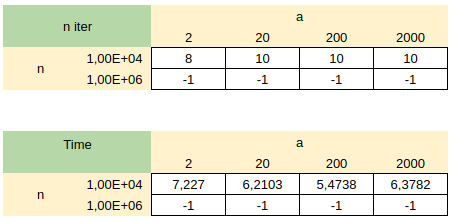
\includegraphics[width=12cm]{table5.png}
	\caption{Starting point of all ones.}
\end{figure*}\\
Results using reduction of the jacobian.
\begin{figure*}[h]
	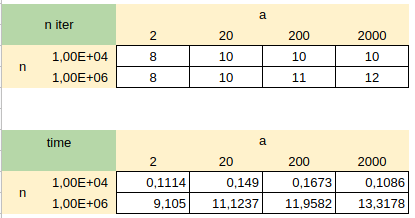
\includegraphics[width=12cm]{table2.png}
	\caption{Starting point of all ones.}
\end{figure*}
\pagebreak
\subsection{Starting configuration b}
Results using LU factorization.\\
\begin{figure}[h]
	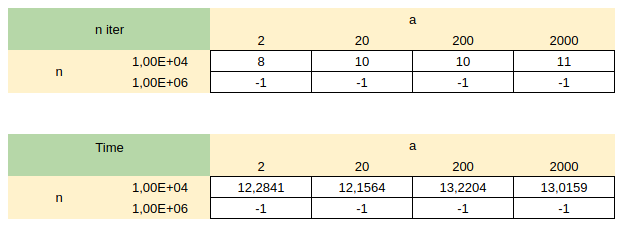
\includegraphics[width=12cm]{table6.png}
	\caption{Starting point of all 100.}
\end{figure}\\
Results using reduction of the jacobian.
\begin{figure}[h]
	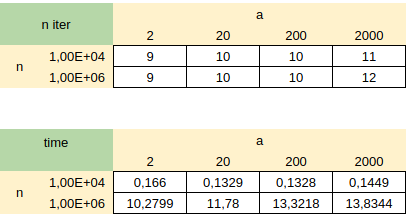
\includegraphics[width=12cm]{table3.png}
	\caption{Starting point of all 100.}
\end{figure}
\pagebreak
\subsection{Starting configuration c}
Results using LU factorization.\\
\begin{figure}[h]
	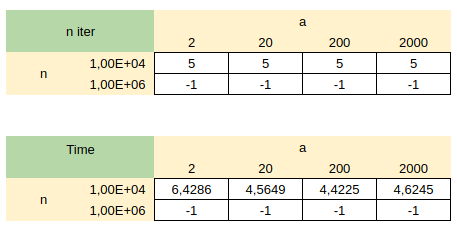
\includegraphics[width=12cm]{table4.png}
	\caption{Starting point as suggested on the book.}
\end{figure}\\
Results using reduction of the jacobian.
\begin{figure}[h]
	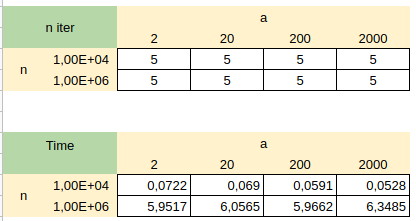
\includegraphics[width=12cm]{table1.png}
	\caption{Starting point as suggested on the book.}
\end{figure}
\pagebreak
\section{Comments}
As we can see, the only difference between the two different approaches is the execution time. This is because the method is the same, I'm just using different ways of computing it...\\
The worse is the starting point, the longer it takes to converge...\\\\
You can find the code I used to solve this problem here: \url{https://github.com/matbun/Num-opt/tree/master/p1/code}.
\end{document}
